% PIR integrationstest

Der er foretaget en integrationstest mellem PIR-sensoren og PIR APIen for at sikre at disse to interagerer korrekt sammen. PIR-sensorens output er sat til P1[1] på PSoCen, hvorefter der er brugt samme testprogram som i modultesten af PIR API. Resultatet ses på figur \ref{lab:test_maaling1} og det kan nu konkluderes at PIR-sensoren og PIR APIen fungerer korrekt sammen, da ISR rutinen går ind og aktiverer testpinen der måles på.

\begin{figure}[H]
\centering
{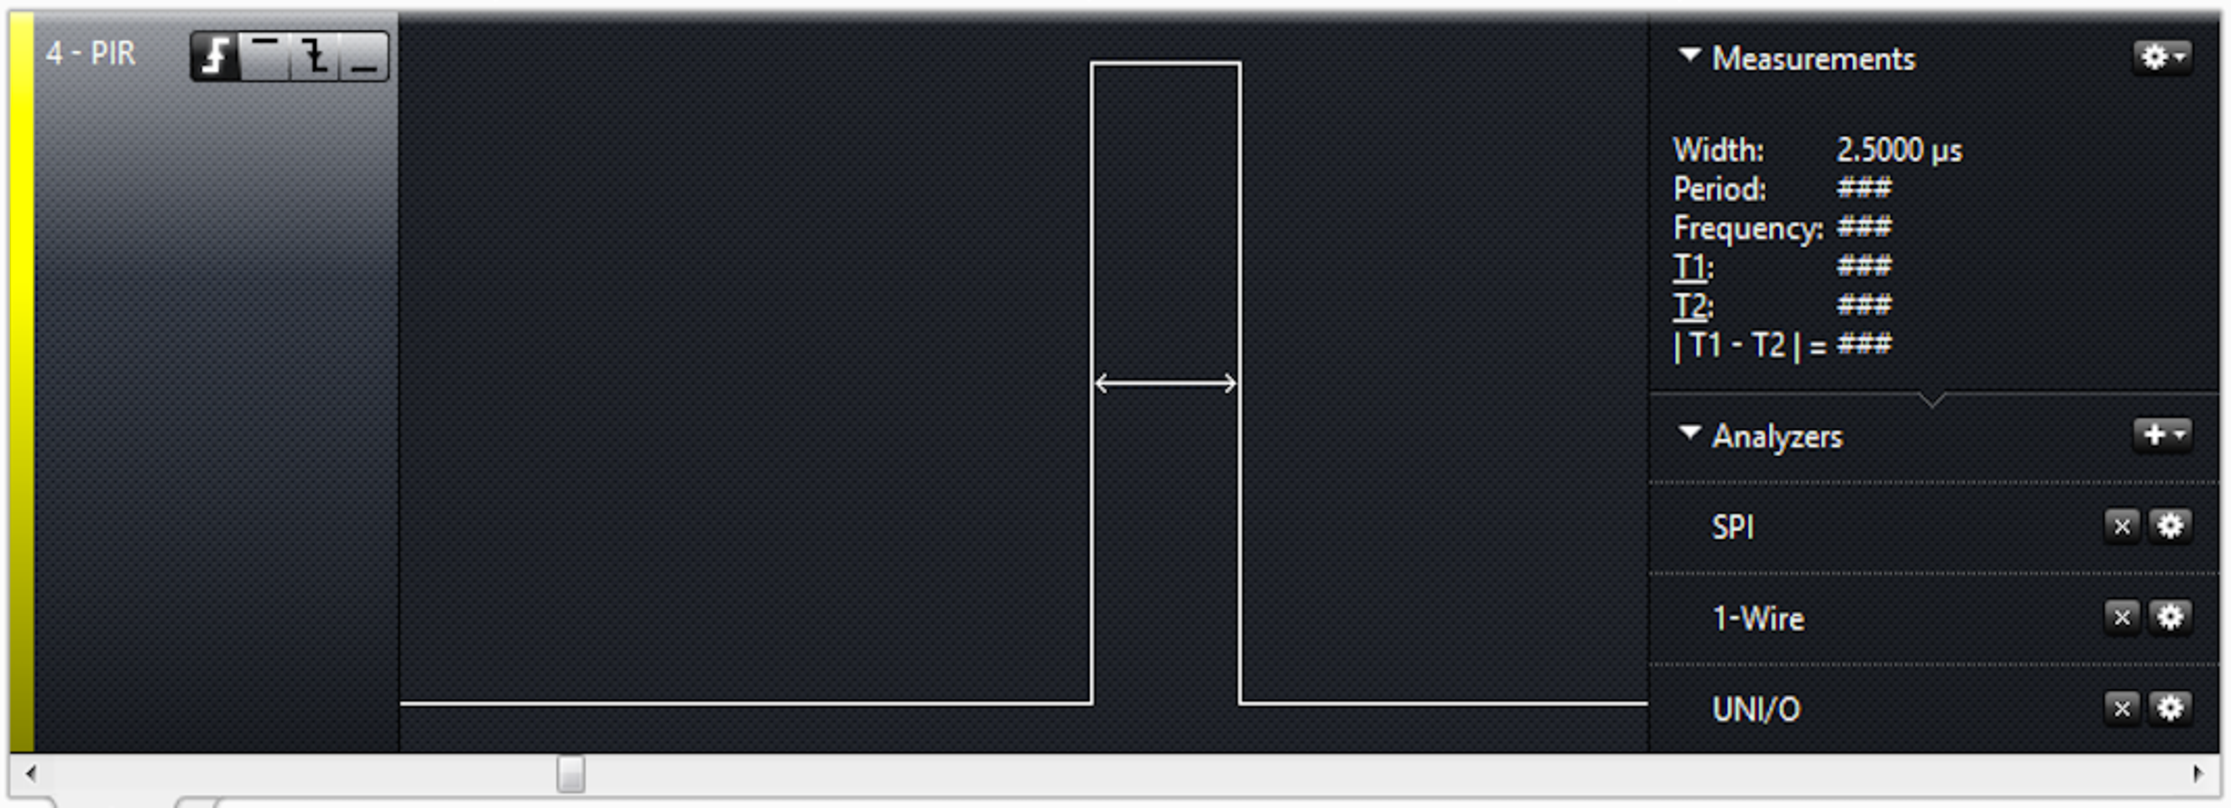
\includegraphics[width=0.60\textwidth]{filer/modultest/billeder/pir_testmaaling}}
\caption{Analysebilledet for PIR aktivering}
\label{lab:test_maaling1}
\end{figure}  